\section{Methodology} \label{sec:methodology}
    
    \subsection{Baseline Degradation model} \label{subsec:baseline_degradation_model}

        Early super-resolution methods commonly generated high-resolution (HR) to low-resolution (LR) samples using predefined degradation techniques, with bicubic downsampling being the most used setting \cite{zhang2018residual}. This kind of synthetic data, while easy to obtain, often results in a domain gap problem, where the data used for training and assessing the model do not come from the same distribution as real data. This gap usually to performance drops when the models implemented in production environments. A possible solution is to synthesize samples with a stochastic degradation model, which includes a set of multiple blurring kernels and several random noises configurations. The larger degradation space grant these models better generalization capabilities and experts be part of the kernel definition process, based on prior knowledge of the degradation process. Unfortunately, the variety of predefined degradation's is still limited and still fail in most applications.

        A degradation model like this one will be used as a baseline for this work.
        

        \subsubsection{Blurring Kernel}

        \begin{figure}[h!]
                \centering
                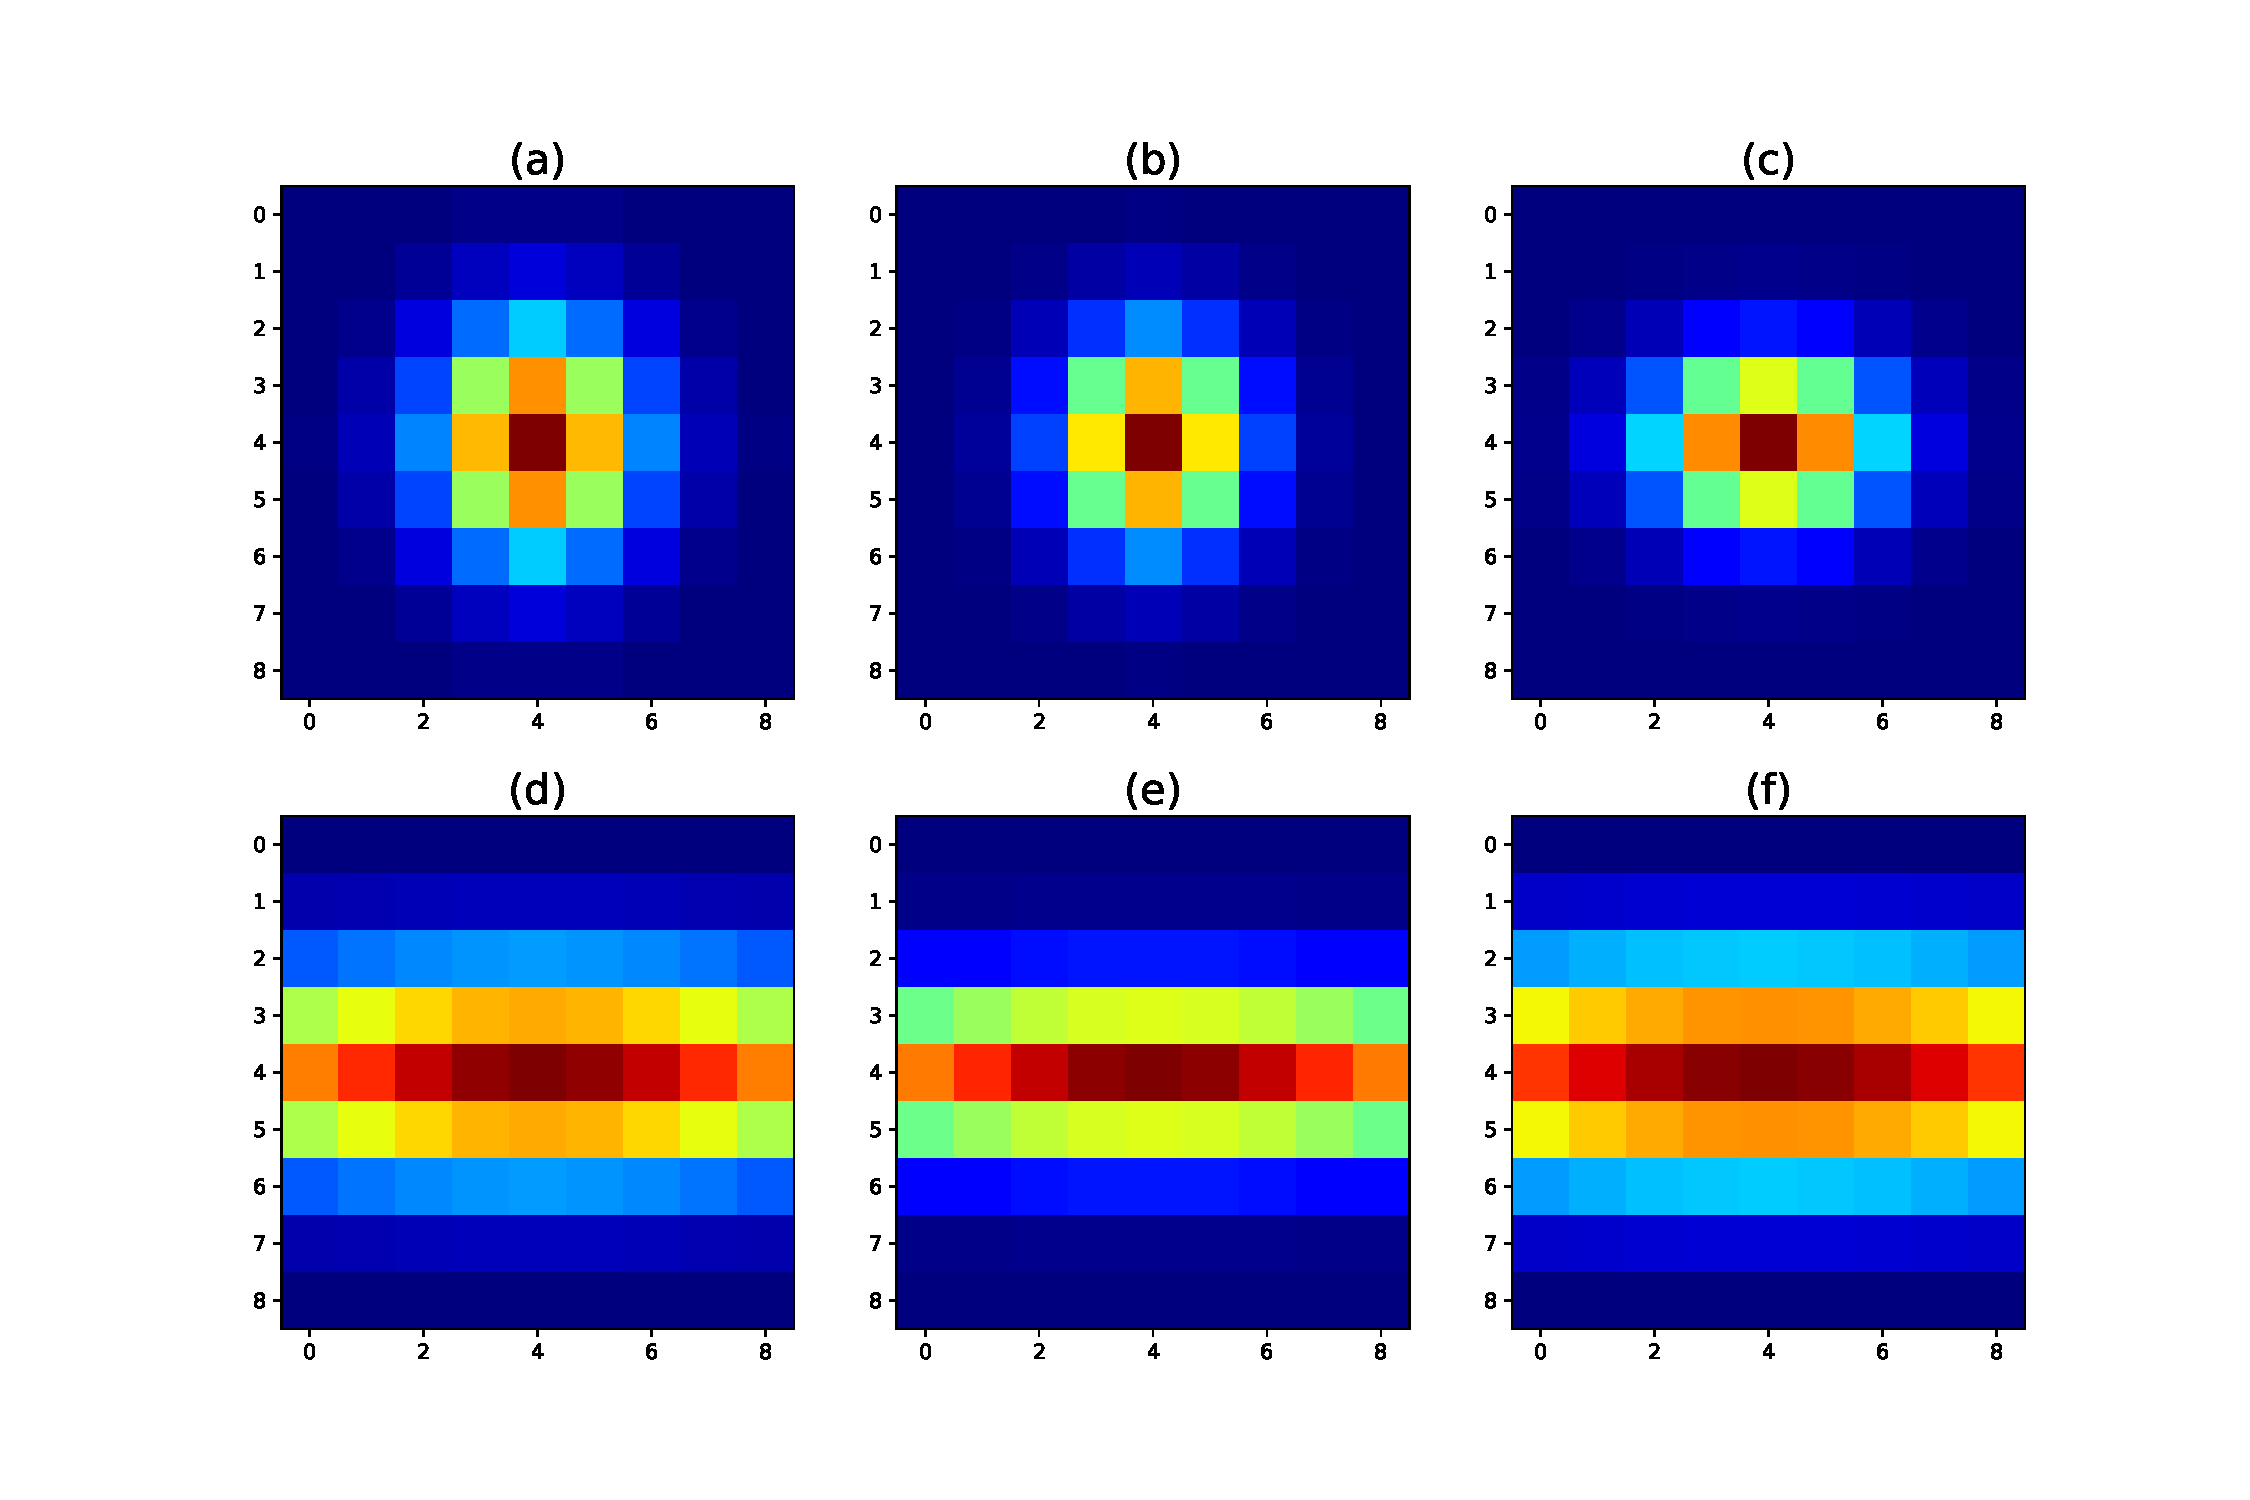
\includegraphics[width=\linewidth]{Includes/4-degradation_kernels.pdf}
                \caption{Example of kernels used in an stochastic degradation model. (a),(b) and (c) are generated using a symmetric variance on the x and y axis. (d) (e) and (f) are generated using an asymmetric variances, resulting in much more anisotropic kernels.}
                \label{fig:4-degradation_kernels}
            \end{figure}

        \begin{figure}[h!]
                \centering
                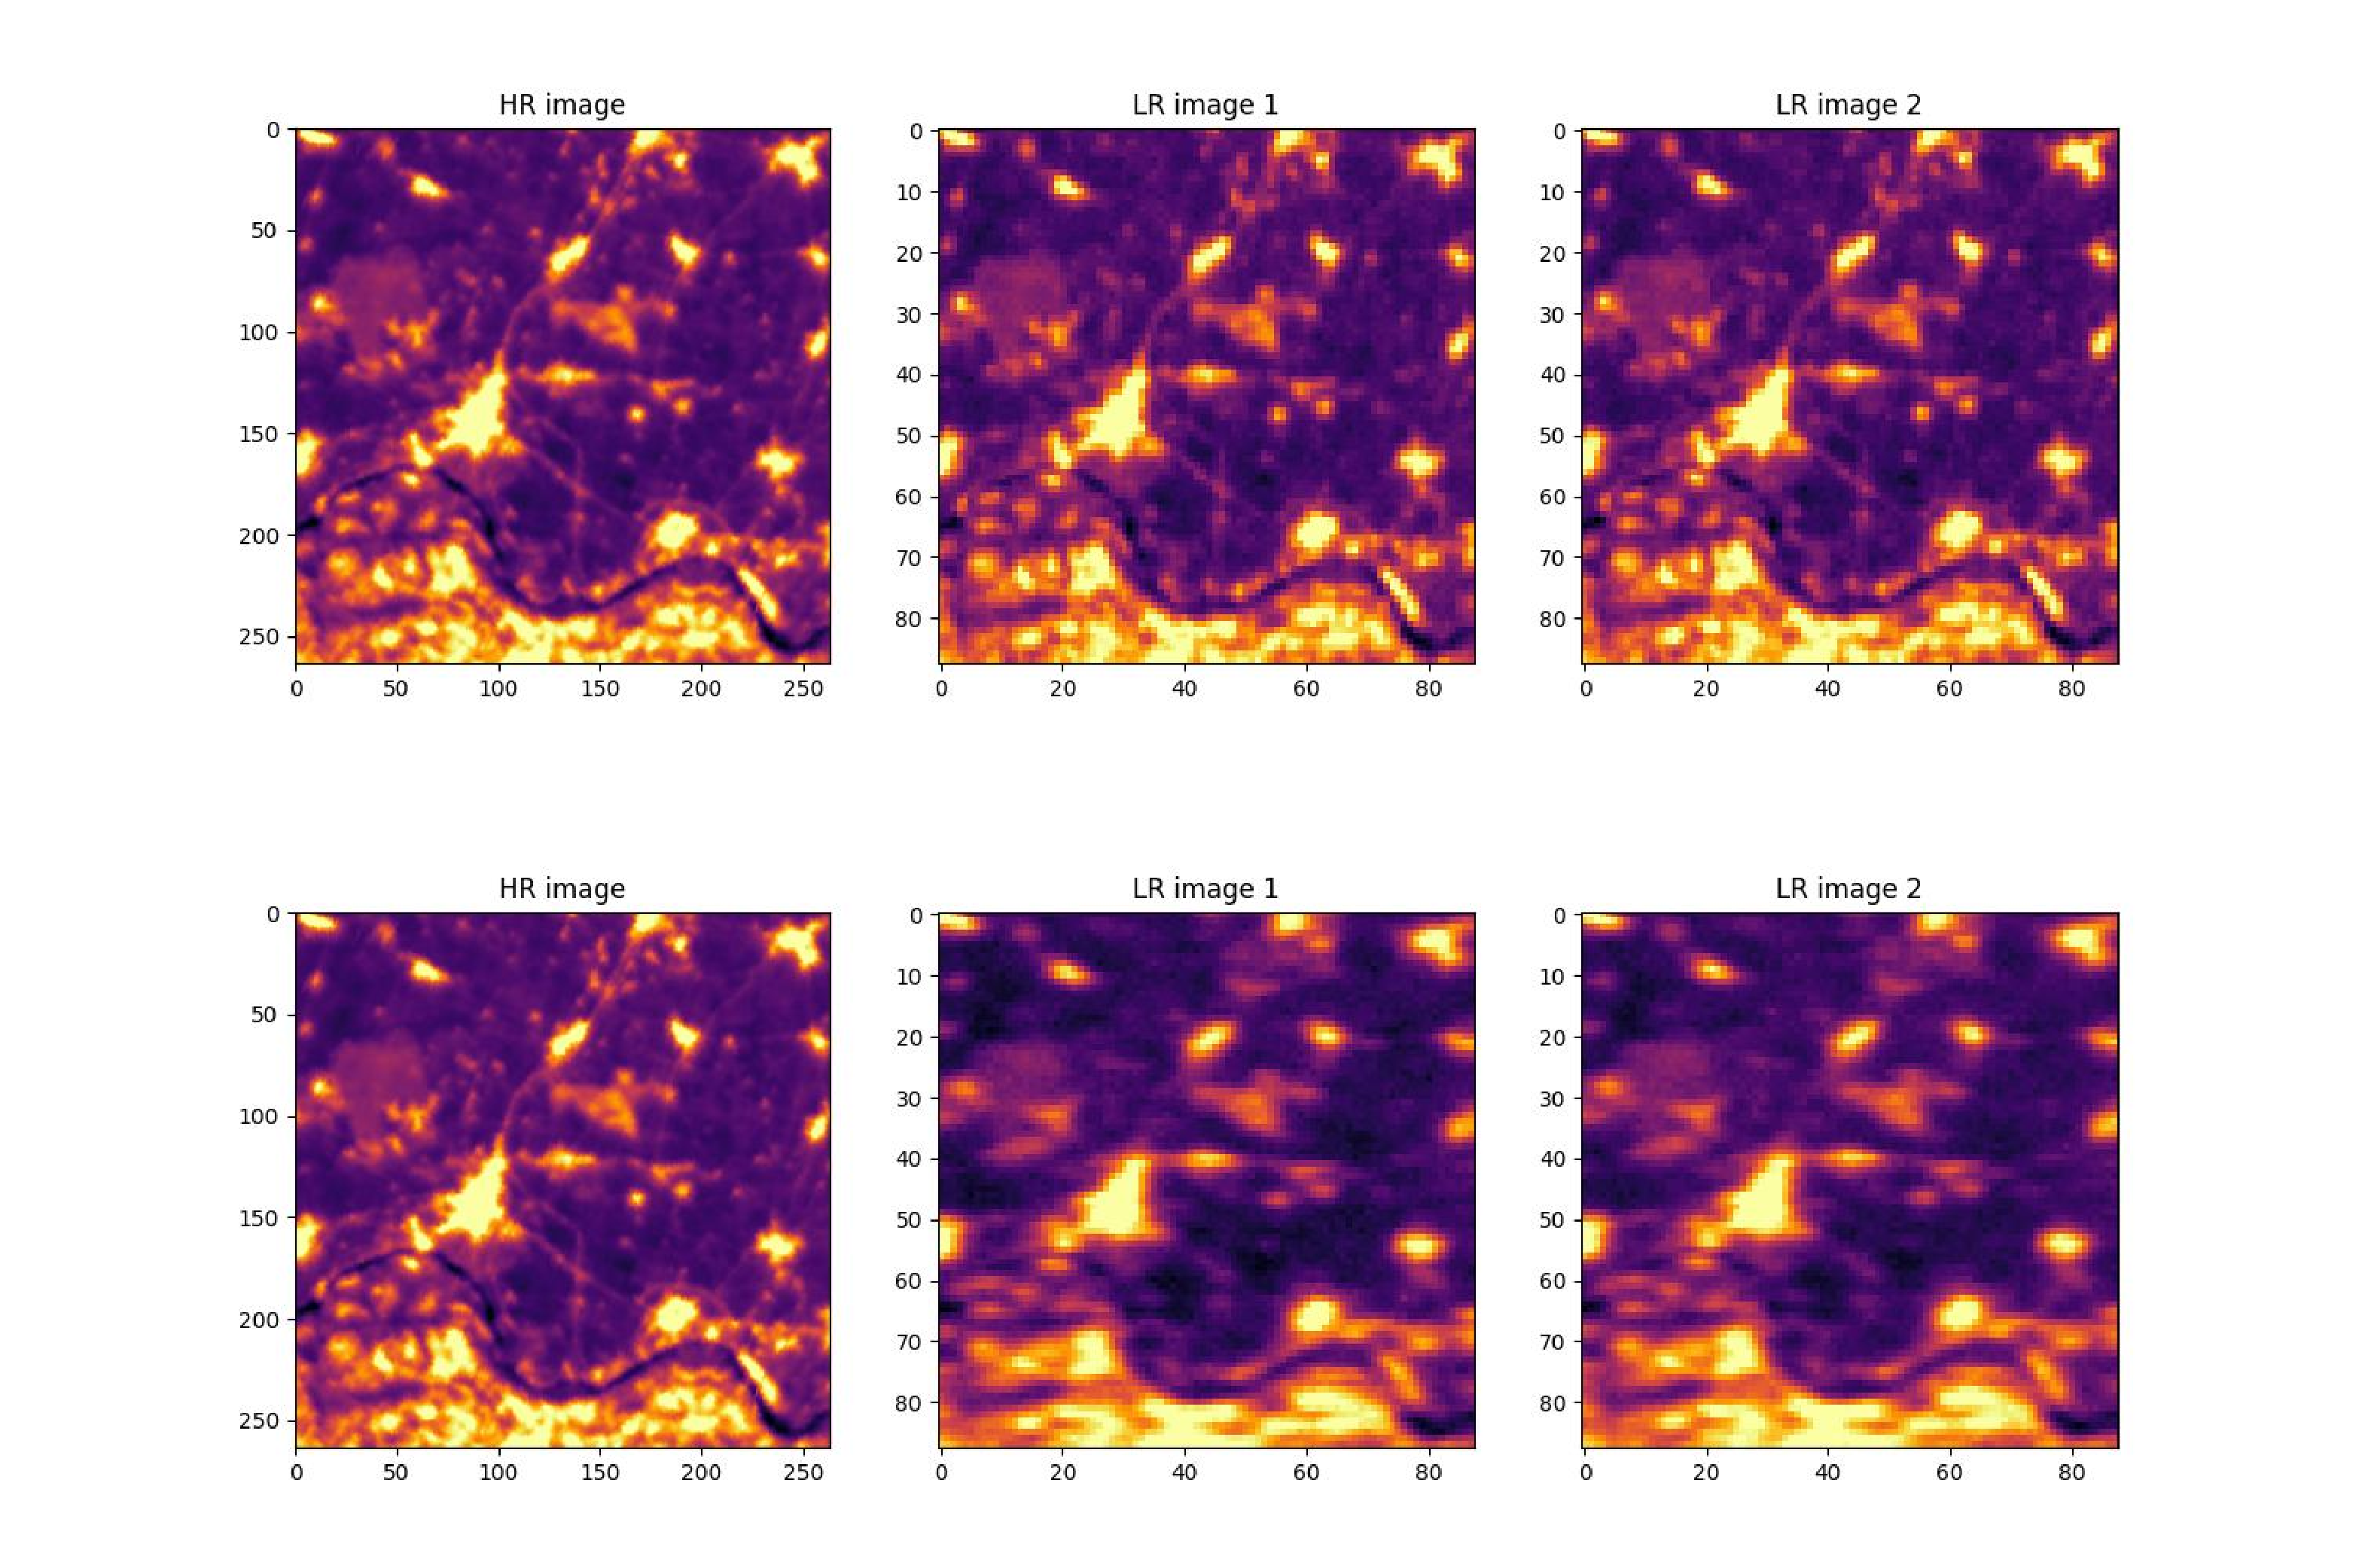
\includegraphics[width=\linewidth]{Includes/4-degradation-kernel-examples.pdf}
                \caption{Effects of different blurring kernels on the HR-LR generation. The upper row contains images generated using blurring kernels with symmetric distributions. The lower rows contains images generated using asymmetric distributions for the variances, resulting in highly anisotropic kernels.}
                \label{fig:4-degradation_kernels}
            \end{figure}
            
        \subsubsection{Radiometric error correction}

        As reported by the ECOSTRESS instrument sheet,\cite{ECOSTRESS2023INSTRUMENT} its nominal radiometric accuracy at 300K is 0.5K. FOREST-2 target radiometric accuracy is 1K. This difference in accuracy should be taken into account. To align these accuracies, we first calculate the additional error required using the following equation:

        \begin{equation}
            e_{\text{forest}} = \sqrt{e_{\text{eco}}^2 + e_{\text{extra}}^2} 
            \label{eq:4-radiometric-error-correction}
        \end{equation}
        
        where $e_{\text{eco}}$ is the ECOSTRESS error, and $ e_{\text{extra}}$ is the additional error required for FOREST-2.
        
        Using the above equation, we find that an additional radiometric error of approximately 0.8660K is needed. The next step involves converting this extra error into a radiance value. This requires calculating the derivative of the Planck equation at 300K, which is done numerically as follows:
        
        \begin{equation}
            \frac{\partial B}{\partial T} = \frac{B(\lambda, T + \delta T) - B(\lambda, T)}{\delta T}
            \label{eq:4-planck-derivative}
        \end{equation}  
        
        By multiplying the results of equations \ref{eq:4-radiometric-error-correction} and \ref{eq:4-planck-derivative}, we can obtain the radiance error for both FOREST LWIR bands. The additional radiance errors for LWIR1 and LWIR2 bands are found to be \(1.5472 \times 10^{-1}\) W/sr/m\(^2\)/\(\mu m\) and \(1.1444 \times 10^{-1}\) W/sr/m\(^2\)/\(\mu m\), respectively.

        The difference in radiances will be split into two components. On one side, the cold Bias represents a systematic error in the measurement, this error acknowledges discrepancies that can be attributed to sensor calibration and atmospheric conditions. On the other side, the random noise accounts for unpredictable fluctuations in the measurement process. It could be due to a variety of sources like electronic noise in the sensor, random atmospheric disturbances, or other stochastic factors. As the extent of each component is not known and to give more variability to this basic degradation model, a random factor $\phi \in [0,1] $ is introduced so that:

        \begin{equation}
        \begin{aligned}
            \varepsilon_{\text{final}} &= (1 - \phi) \times \varepsilon_{\text{radiance}} + \phi \times \eta \times \varepsilon_{\text{radiance}} \\
            \eta & \sim \mathcal{N} (0,1)
        \end{aligned}
        \end{equation}    

        The effects of the error correction is shown in Fig. \ref{fig:4-radiometric_noise_example}. As the target radiometric error increases with respect to ECOSTRESS scenes, the loss of information is more noticeable.


        \begin{figure}[h!]
            \centering
            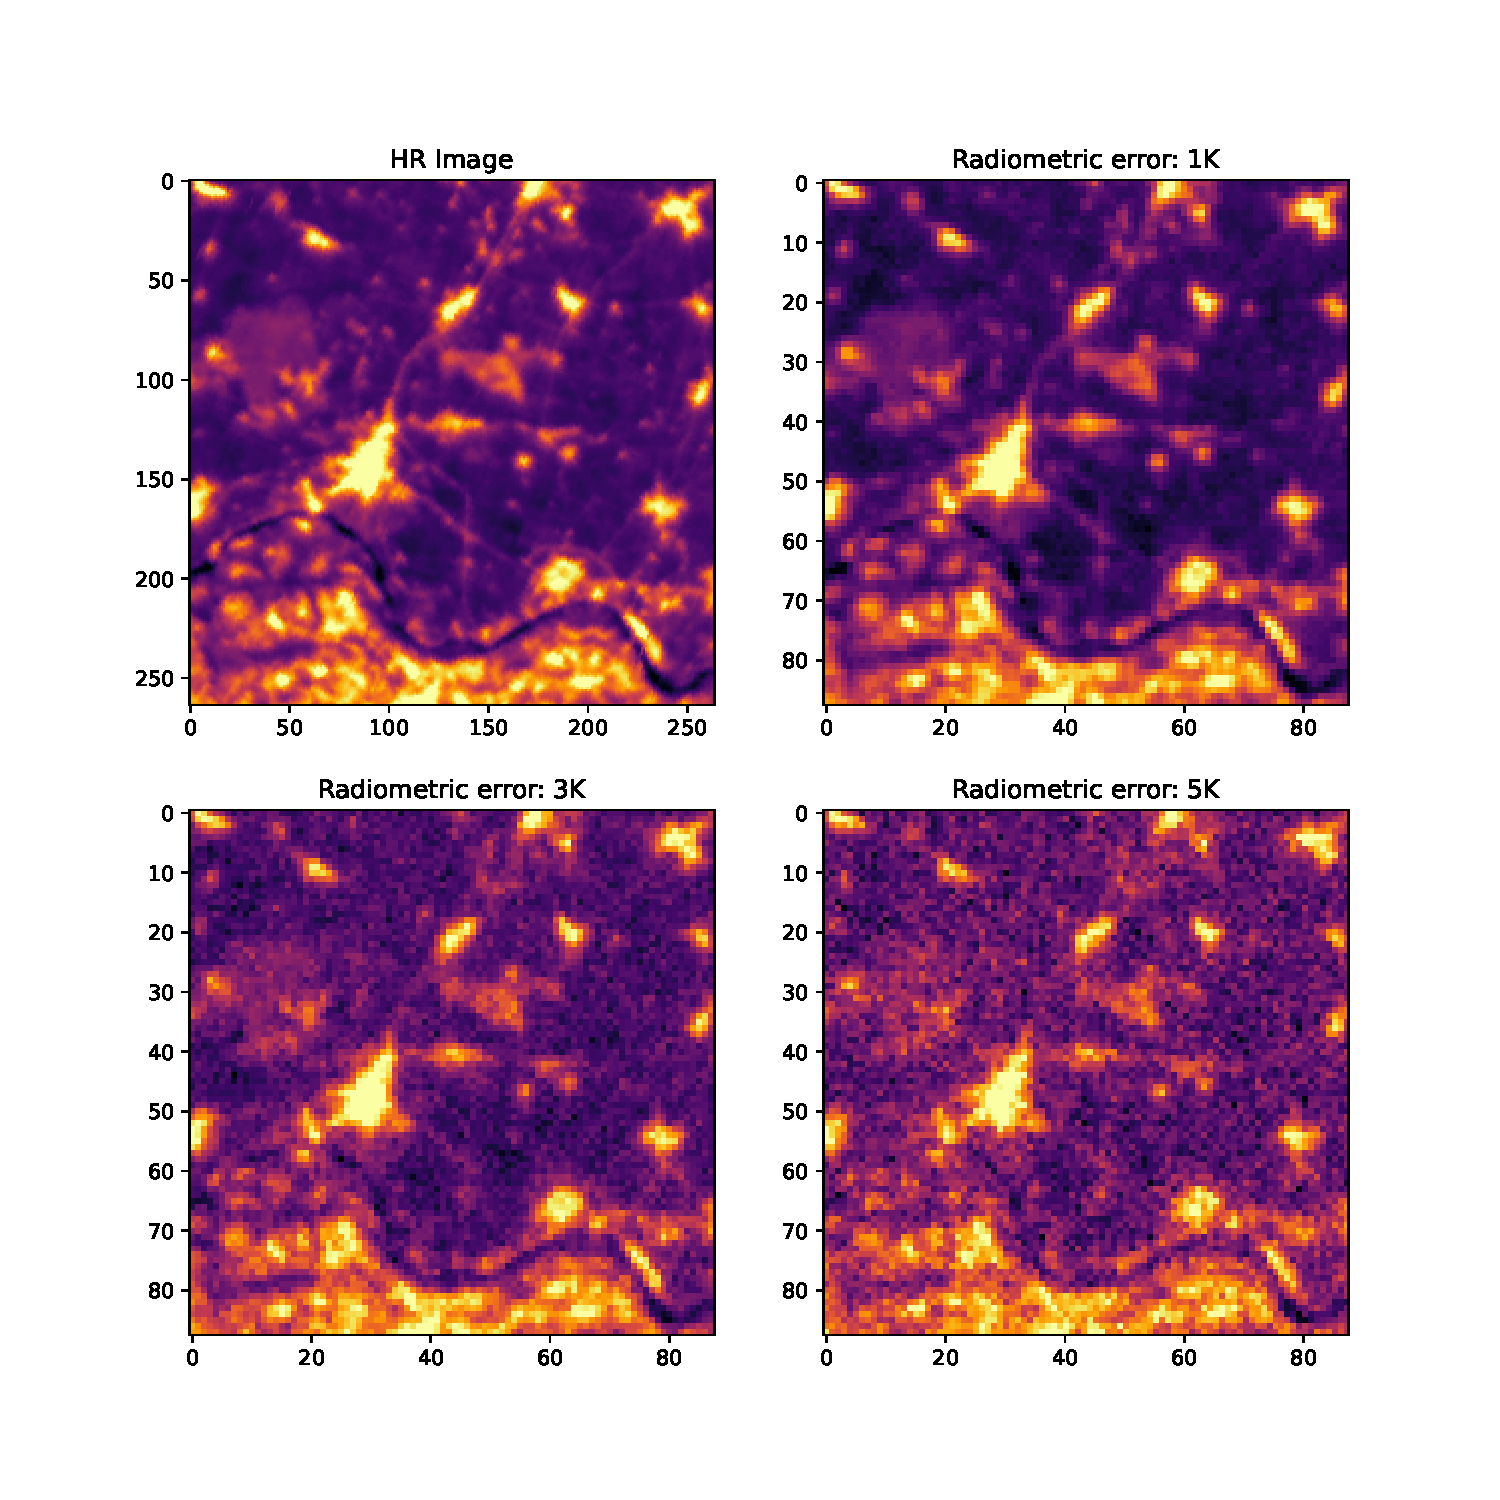
\includegraphics[scale=0.55]{Includes/4-radiometric_noise_example.pdf}
            \caption{Effects of different radiometric error corrections on the HR-LR generation.}
            \label{fig:4-radiometric_noise_example}
        \end{figure}
        
    \subsection{Models Architecture}
    
        \subsubsection{SRResNet}

            Introduced in 2017 \cite{ledig2017photorealistic}, SRResnet leverages on residual networks \cite{he2015deep} that employ skip connections to solve the super resolution task. The architecture is detailed in Fig. \textbf{CITE}. Specifically, 16 residual blocks consisting two convolutional layers, followed by batch-normalization layers and ParametricReLU activation functions. The convolutional layers have 3x3 kernels and 64 feature maps. To increase the resolution of the input image, two trained sub-pixel convolution layers are used.

            As this work focuses on having super resolved images with high physical consistency and not on the perceptual superiority of the images, improvements introduced in the publications like the Generative Adversarial Network (SRGAN)  and the perceptual loss for gradient calculation are not used.
        

        \subsubsection{RAMS}
        \subsubsection{Probabilistic Degradation Model}

            \begin{figure}[h!]
                \centering
                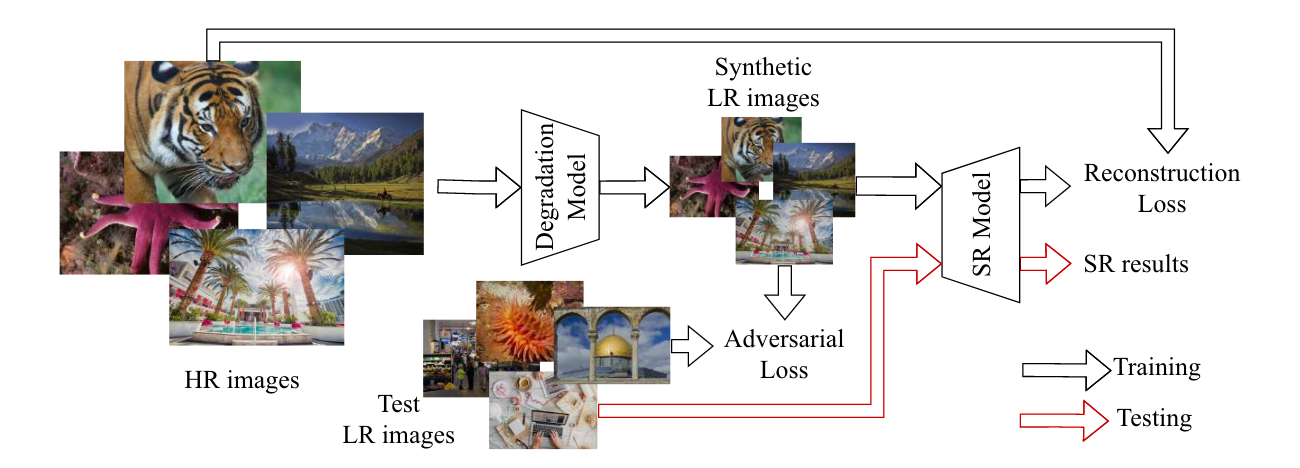
\includegraphics[scale=0.55]{Includes/3-GAN-degradation-model.png}
                \caption{In Degradation-learning-based methods like this one, 
                         adversarial training is used to encourage the degradation model to produce images in the same domain with the target domain (test images).
                         Source \cite{luo2022learning}.}
                \label{fig:3-GAN-degradation-model}
            \end{figure}

            \paragraph{Kernel Model}
            \paragraph{Noise Model}
            \paragraph{Discriminator}


    \subsection{Performance Metrics}

        \subsubsection{Referenced image quality metrics}

        
        
    
            \paragraph{Adjusting measures to a multi-image framework}
    
            In order to calculate the losses and performance metrics, the generated test images (SR) are compared against the ground truth high resolution images (HR). Additional changes should be introduced in a MISR environment \cite{martens2019superresolution}. First, minor shifts on the contents of the pixels are expected and they should have some tolerance to small pixel-translations in the high-resolution space by evaluating on a sliding cropped image. That means, looking for a displacement of SR by at most d pixels in each direction that minimizes the error. An example of how this is applied in a loss that needs to be minimized can be found in Eq. \ref{eq:4_adjusted_metrics}
    
            \begin{equation}
               \mathcal{L}^* ( I^{HR}, I^{LR}, d) = \min_{u,v \in [0,2d]} \mathcal{L} ( I^{HR}_{u,v}, I^{SR}_{u,v})
            \label{eq:4_adjusted_metrics}
            \end{equation}
    
            Additionally, commonly used metrics punish biases as much as noise in the reconstruction. For example, if $I^{SR} = I^{HR} + \epsilon$, where $\epsilon$ is a constant bias, a perfect reconstruction of $I^{SR}$ is possible if $\epsilon$ is known. A quality metric should award  a high score in super-resolutions with this characteristics in comparison to the introduction of noise and information loss. Metrics like L2/L1 losses and PSNR do the exact opposite and should have a bias compensation like the following: 
    
            \begin{equation}
                \begin{aligned}
                    \mathcal{L}^* ( I^{HR}, I^{LR}, d) = \min_{u,v \in [0,2d]} \mathcal{L} ( I^{HR}_{u,v}, (I^{SR}_{u,v}+b)) \\
                    b = \frac{1}{(W - d)(H - d)} \sum_{x,y} \left( I^{HR}_{u,v} - I^{SR}_{u,v} \right)
               \end{aligned}
            \end{equation}
    
            \noindent where $W$ and $H$ represent the width and height of the image, respectively.
    

        

        \subsubsection{No-reference Image quality metrics}

        As a result, NIQE has found widespread use across various domains of image processing, including restoration, compression, and enhancement, where it serves as a standard for the performance of algorithms, particularly in the realm of image super-resolution.

        \paragraph{Naturalness Image Quality Evaluator (NIQE)}\mbox{} \\

        
            The Naturalness Image Quality Evaluator (NIQE) \cite{niqe} is a no-reference image quality assessment metric that quantifies the perceptual quality of images based on their naturalness. Unlike traditional metrics that require a reference image for comparison, NIQE operates on the principle that pristine natural images exhibit specific statistical properties that can be quantified to establish a benchmark for quality assessment. NIQE employs a model based on a multivariate Gaussian distribution, characterized by a mean vector and covariance matrix, to represent the statistical attributes of a natural image's visual patterns. To assess the quality of an image, NIQE extracts a corresponding set of features and evaluates their deviation from this statistical model using the Mahalanobis distance. This distance measures the divergence of the image's features from those typical of high-quality natural images. A lower value suggests that the image closely resembles the statistical properties of natural images, indicating higher perceived quality.
            
            However, NIQE provides an objective measure of image quality that aligns with the naturalness of human visual perception, and is not able to quantify the physical consistency of a generated image.
        \paragraph{BRISQUE}

        \subsubsection{Frequency Domain Analysis} \label{subsubsec:frequency_domain_analysis}
        
        The Fourier transform is widely used to analyze the frequency content in signals.  It can be applied to multidimensional signals such as images, where the spatial variations of pixel-intensities have a unique representation in the frequency domain. Super-resolution objective is to reconstruct missing high frequency components from a downscaled image. The expectation of a good SR algorithm is to amplify the high frequency components compared to a baseline like bicubic interpolation, while keeping noise at bay. The Fourier components provide global information about the image, as opposed to local information represented by pixel values in the spatial domain \cite{fuoli2021fourier}. 

        
        Utilizing the Fast Fourier Transform (FFT), we convert the pixel intensity values of super-resolved images into a spectrum where each point represents a specific frequency contained in the spatial domain. The FFT is shifted so that the zero-frequency component is at the center of the spectrum. The resulting magnitude, after applying a logarithmic transformation, reveals the energy distribution across various frequencies. This is visualized in grayscale, where the intensity corresponds to the amplitude of the frequency components.
        
        A radial profile of the FFT magnitude provides insights into how different spatial frequencies contribute to the image content in the vertical and horizontal direction. The radial profile is a function of the average intensity of frequencies at a given radius from the center of the Fourier transform.
        
        The average of the FFT magnitude is calculated for concentric circles of increasing radii, capturing a statistic of the frequency components for every direction. This metric serves as a benchmark for evaluating the performance of SR techniques against traditional interpolation methods such as bicubic interpolation.

        Spatial frequency within an image context refers to the periodicity of the intensity variation over spatial dimensions, typically quantified in cycles per pixel. The central region of the frequency domain, after the shift operation, denotes the zero frequency. In contrast, the extremities of the domain delineate the highest frequencies, constrained by the image's discrete sampling rate.

        To quantitatively interpret these spatial frequencies, a radial-to-frequency mapping is necessary. This mapping accounts for the Nyquist frequency, which is delineated as half the sampling rate of the discrete imaging grid and acts as a threshold to prevent frequency aliasing.

        The conversion from a given radius in the FFT output to the corresponding spatial frequency is formalized as:

        \begin{equation}
            f(r) = \frac{r}{\frac{N}{2}} \cdot f_{\text{Nyquist}},
        \end{equation}

        where \( f(r) \) signifies the spatial frequency associated with radius \( r \), \( N \) represents the FFT image dimension, assuming a square configuration, and \( f_{\text{Nyquist}} \) the Nyquist frequency, which is 0.5 cycles per pixel in this case.

        Through FFT we acquire a depiction of the frequency-based amplification or attenuation attributable to the SR techniques. Analyzing these profiles displays the ability of SR models for detail enhancement. However, it is important to note that this method does not account for any noise or artifacts generated by the SR, and should be used in combination to other supervised metrics.

        \begin{figure}[h!]
            \centering
            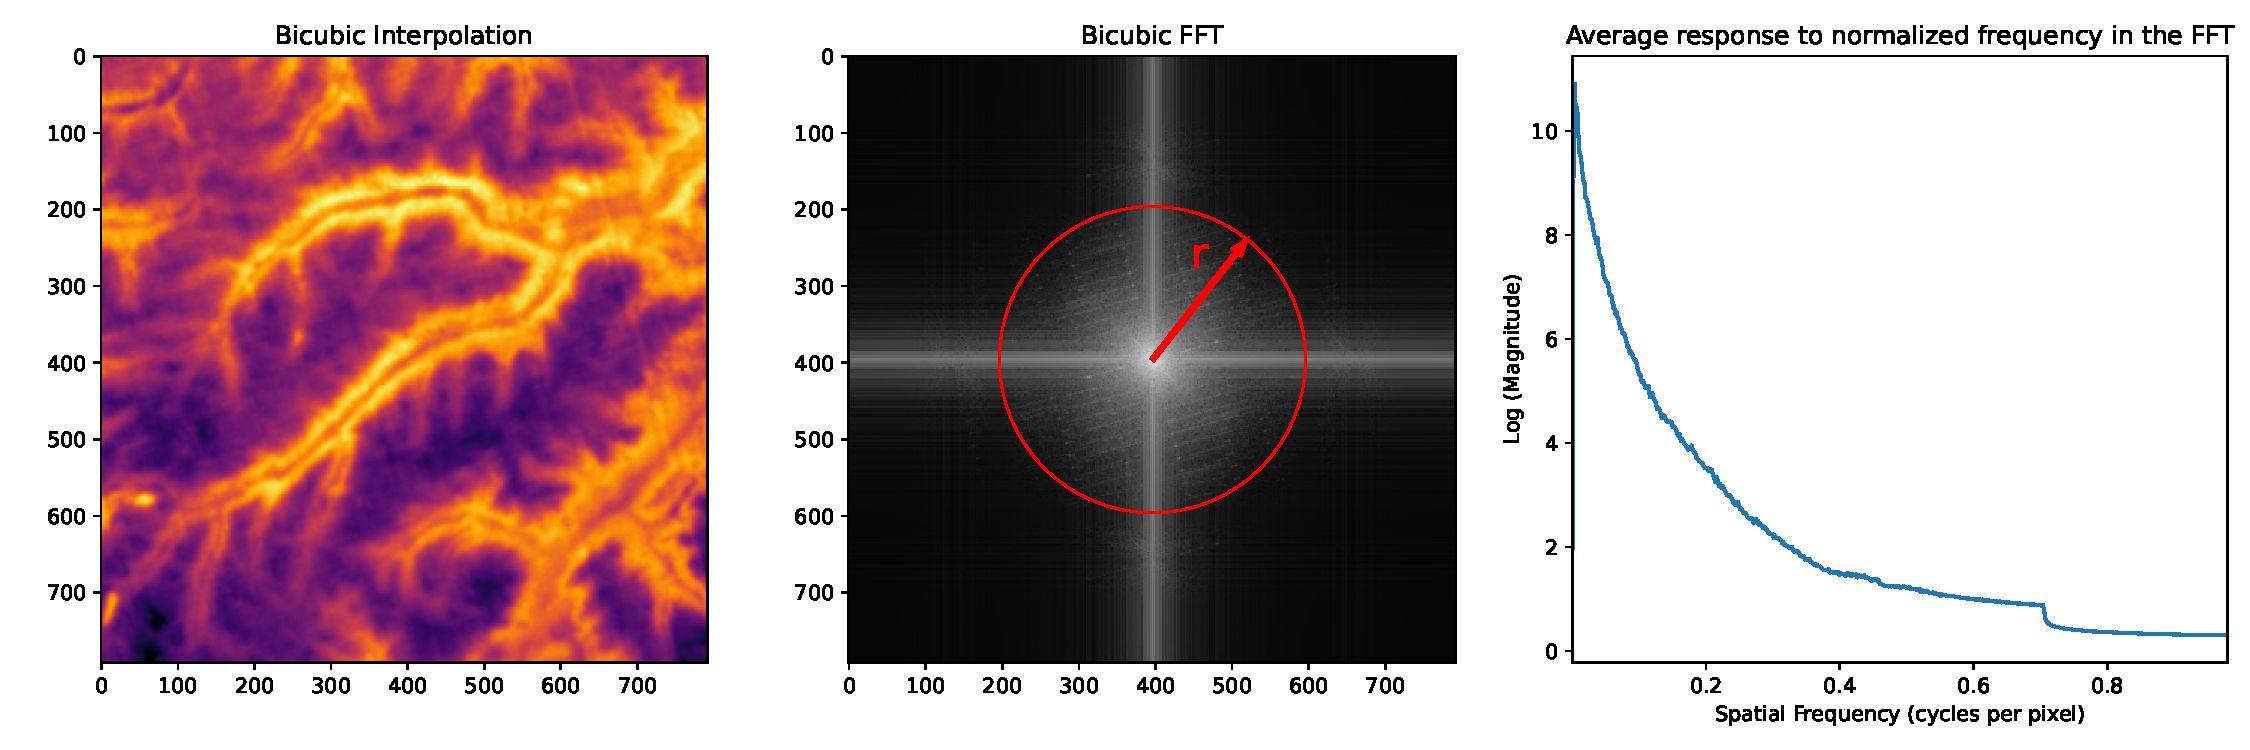
\includegraphics[width=\linewidth]{Includes/4-frequency-analysis.pdf}
            \caption{Steps of the frequency domain analysis. The Center image shows the log magnitude of the shifted FFT of a bicubic upsampled FOREST scene and an example of a radial profile, the average of all the points that have the same $r$ is calculated. The right image displays the log magnitude obtained for every radial profile, translated into spatial frequency.  }
            \label{fig:4-frequency-analysis}
        \end{figure}

        \subsubsection{Gradient Distribution analysis}


        An alternative way of analyzing super-resolution results is by looking at the gradients of the images. HR images are sharper and thus each pixel has higher gradients magnitude with respect to both directions than their LR counterparts. A super-resolution algorithm should increase the sharpness of the edges, resulting in a gradient distribution that aligns more closely with that of the genuine HR image. An approximation of the gradients can be estimated by doing 2d convolutions between an image and the so called Sobel kernels displayed in Eq. \ref{eq:4-sobel-operators} \cite{Sobel1990AnI3}. These kernels are designed to respond maximally to edges running vertically and horizontally relative to the pixel grid.
        
        \begin{equation}
            \begin{array}{ccc}
            \hat{G}_x = \begin{bmatrix}
            -1 & 0 & +1 \\
            -2 & 0 & +2 \\
            -1 & 0 & +1
            \end{bmatrix}
            &
            \quad
            &
            \hat{G}_y = \begin{bmatrix}
            +1 & +2 & +1 \\
             0 &  0 &  0 \\
            -1 & -2 & -1
            \end{bmatrix}
            \end{array}
            \label{eq:4-sobel-operators}
        \end{equation}
    
         The kernels can be applied separately to the input image to produce the component of the gradient in each orientation $G_x$ and $G_y$. The magnitude of the gradient  is given by: 
         \begin{equation}
             |G| = \sqrt{G_x^2 + G_y^2}
             \label{eq:4-gradient_magnitude}
         \end{equation}

         The gradient magnitude histograms of the results of different super-resolution algorithms will be assessed, there by quantifying the enhancement in edge sharpness.  This histogram provide insights into the frequency and intensity of the edges within an image. A better SR model should demonstrate a histogram with higher frequencies of larger gradient magnitudes, indicating sharper edges. It is important to note that this analysis is unsupervised and disregards the effect of noise and artifacts introduced during the super-resolution process and should be considered in combination with other supervised metrics like PSNR.

         \begin{figure}
             \centering
             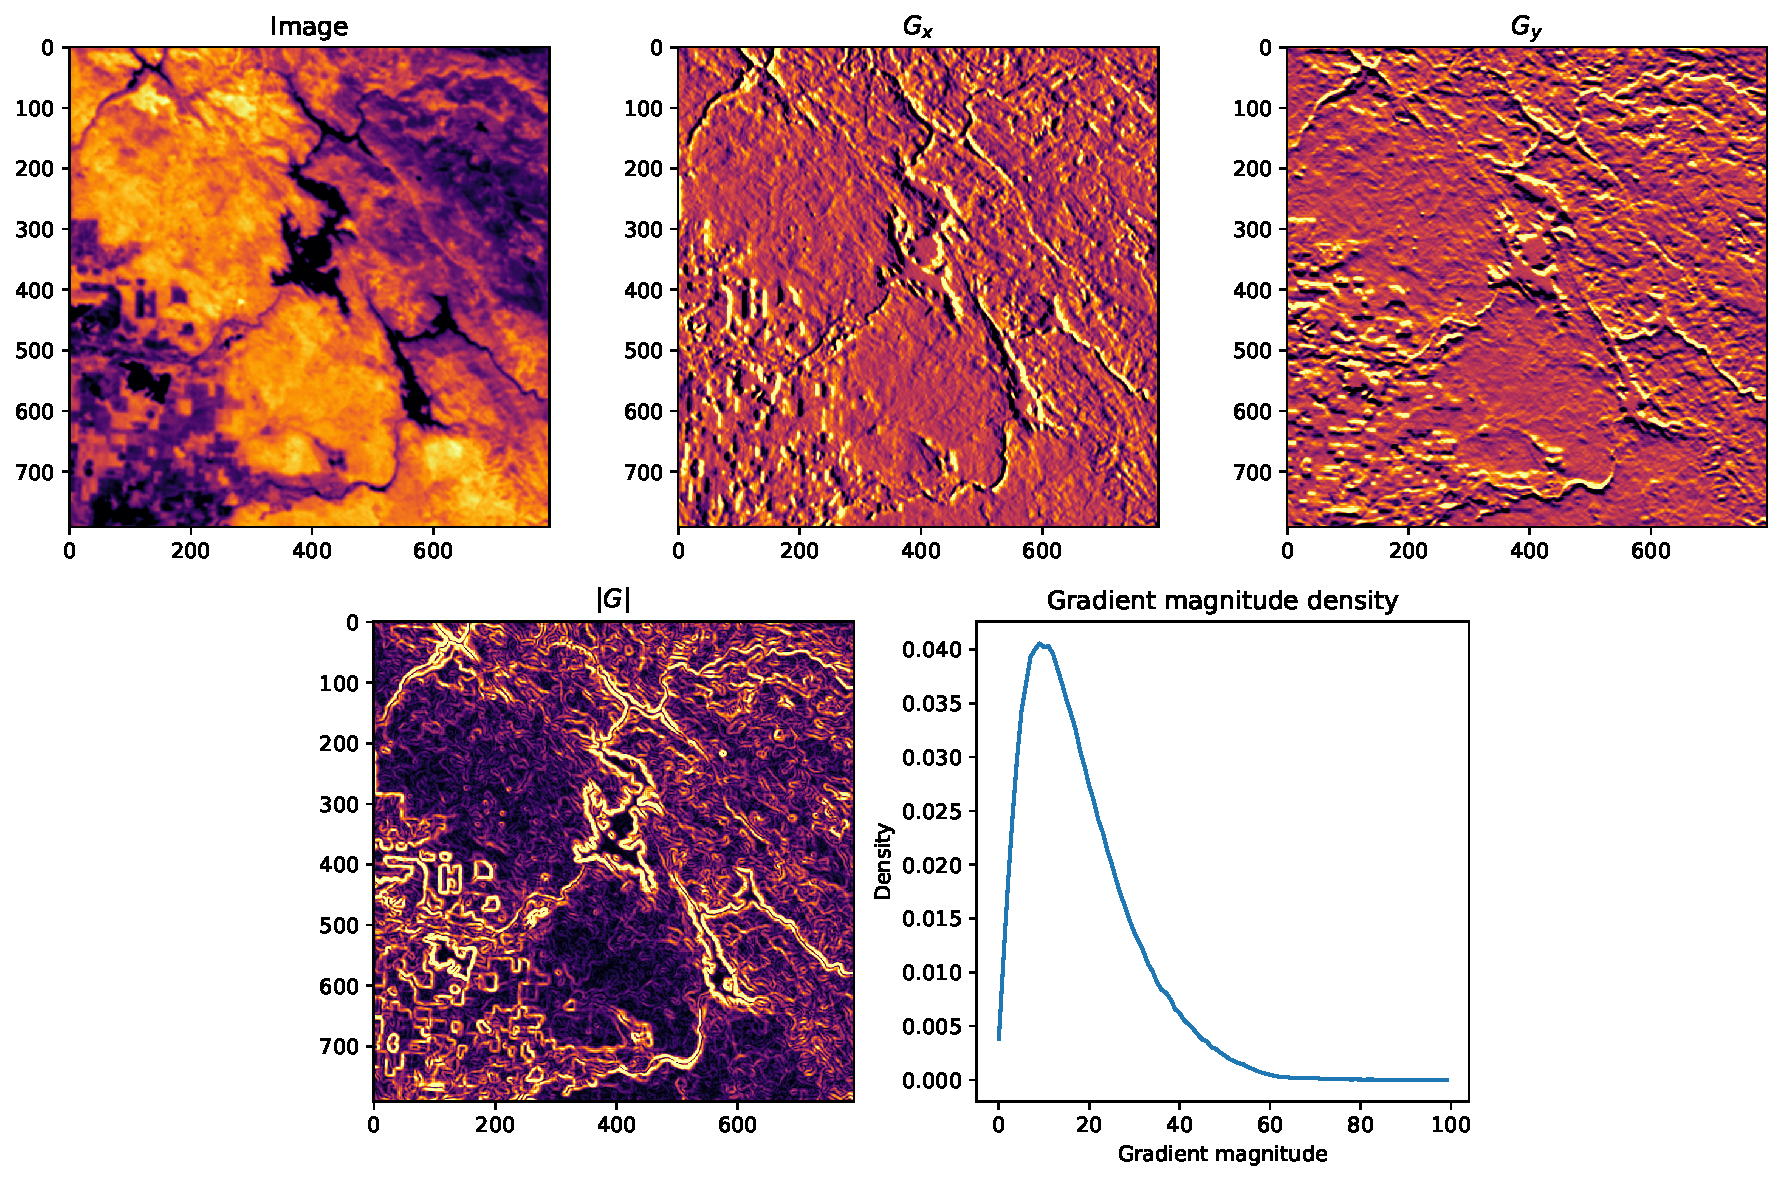
\includegraphics[width=\textwidth]{Includes/4-gradient-analysis.pdf}
             \caption{Steps to obtain a gradient magnitude density. Using the sobel operators, $G_x$ and $G_y$ are obtained from an image. The magnitude $|G|$ of each pixel is calculated using Eq. \ref{eq:4-gradient_magnitude}. The density can be estimated afterwards, using 100 bins in this case.}
             \label{fig:4-gradient-analysis}
         \end{figure}

         

\clearpage

        

        
        
